\subsection{舆论演化图上的接触过程}
\begin{frame}{舆论演化图上的接触过程}
    出发点:不同国家对于防疫策略的反应是不同的。以对戴口罩的反应为例:
    \begin{itemize}
        \item 舆论环境下,初始有一定比例$u$的人愿意戴口罩,一部分人不愿意戴
        \item 他们的意愿与社交关系也会共同演变在这个时期改变,戴->不戴、不戴->戴、短期内不交往了的\textit{速率}分别是$\beta_1$, $\beta_2$, $1-\beta_1-\beta_2$
        \item 最终会产生戴-戴,不戴-不戴的组团。
        \item 决定疾病传播阈值的不只是流行病本身,也是人群交往密度和社交关系
    \end{itemize}
\end{frame}

\begin{frame}{舆论演化图上的接触过程}
    \begin{figure}[htbp]
\centering
\subfigure{
\begin{minipage}[t]{0.25\linewidth}
\centering
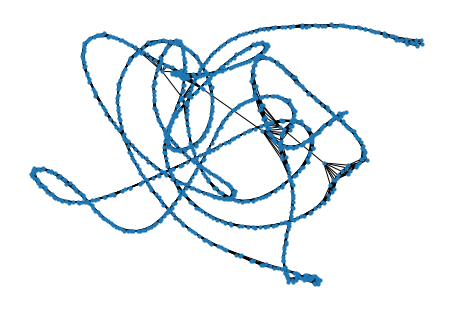
\includegraphics[width=1in]{pics/sw.png}
\caption{Original graph.}
\end{minipage}%
}%
\subfigure{
\begin{minipage}[t]{0.25\linewidth}
\centering
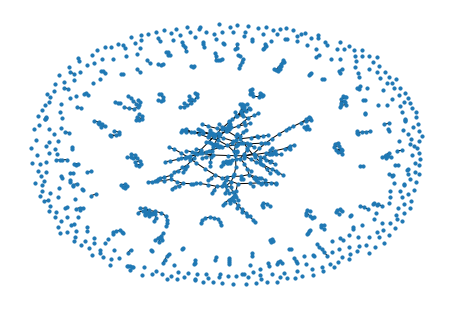
\includegraphics[width=1in]{pics/sw-rw.png}
\caption{Evolving}
\end{minipage}%
}%
\subfigure{
\begin{minipage}[t]{0.25\linewidth}
\centering
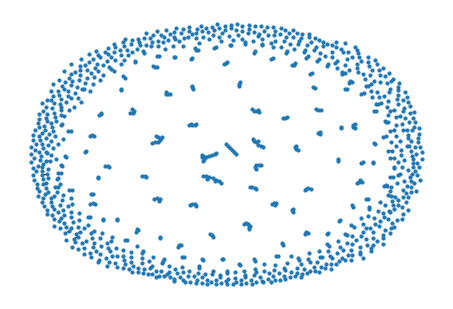
\includegraphics[width=1in]{pics/promasks.png}
\caption{Pros.}
\end{minipage}
}%
\subfigure{
\begin{minipage}[t]{0.25\linewidth}
\centering
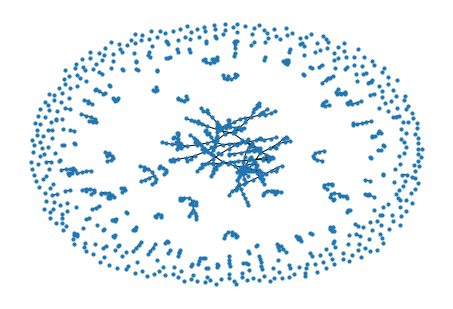
\includegraphics[width=1in]{pics/conmasks.png}
\caption{Cons.}
\end{minipage}
}
\centering
\end{figure}
\end{frame}

\begin{frame}{结果}
    \begin{itemize}
        \item 重要指标的差异性 \vspace{0.5cm}
        \item 流行条件、流行病阈值差异性\vspace{0.5cm}
        \item 形成了牢固连接的中心和临时孤立的节点,这些节点由重连而迅速重新连接\vspace{0.5cm}
        \item 二分岔的混沌状态\vspace{0.5cm}
    \end{itemize}
\end{frame}



\subsection{停工/复工博弈}
\begin{frame}{停工/复工博弈}
    Considering  a  natural  trade-off  of  commuting  patterns  and  epidemics  in  cities,  we  propose a spatial model to suggest which companies should let their employee to go to workplaces.  Our model incorporate demographic noises and spatial interactions in their effects on contagion rate, so that the back-to-work transition can be explicitly determined by heterogeneity of population distributions.
\end{frame}

\subsection{通勤模式对城市空间中疾病传播的影响}

\begin{frame}{通勤模式对城市空间中疾病传播的影响}
    本次抗疫过程中,群体层面主要的限制手段是限制个体出行。实际作用是减小了大部分人的活动半径。需要注意的是,该措施同时会使得局部交互有较大提升。本研究试图探究缩小活动尺度带来的非线性效应。
    
    \vspace{0.5cm}
    
    我们提出了一个基于复杂人口分布的SIER模型,该模型中,每个结点的人口数将不再固定,每个结点的状态将由总人口和患病人口比例两个量来决定。传播规律除了结点间传播之外,还有结点内的高速传播,以模拟小区传播的过程。
    
    \vspace{0.5cm}
    
    在人口的高度异质性假设下,本研究试图证明限制出行并不一定是最优解,而是在小区传播出现之前/患病比例比较低的时期的较优解。%在某些时期,流行病传播与出行限制关系不大。
\end{frame}
\begin{frame}{通勤模式对城市空间中疾病传播的影响}
    \begin{figure}
        \centering
        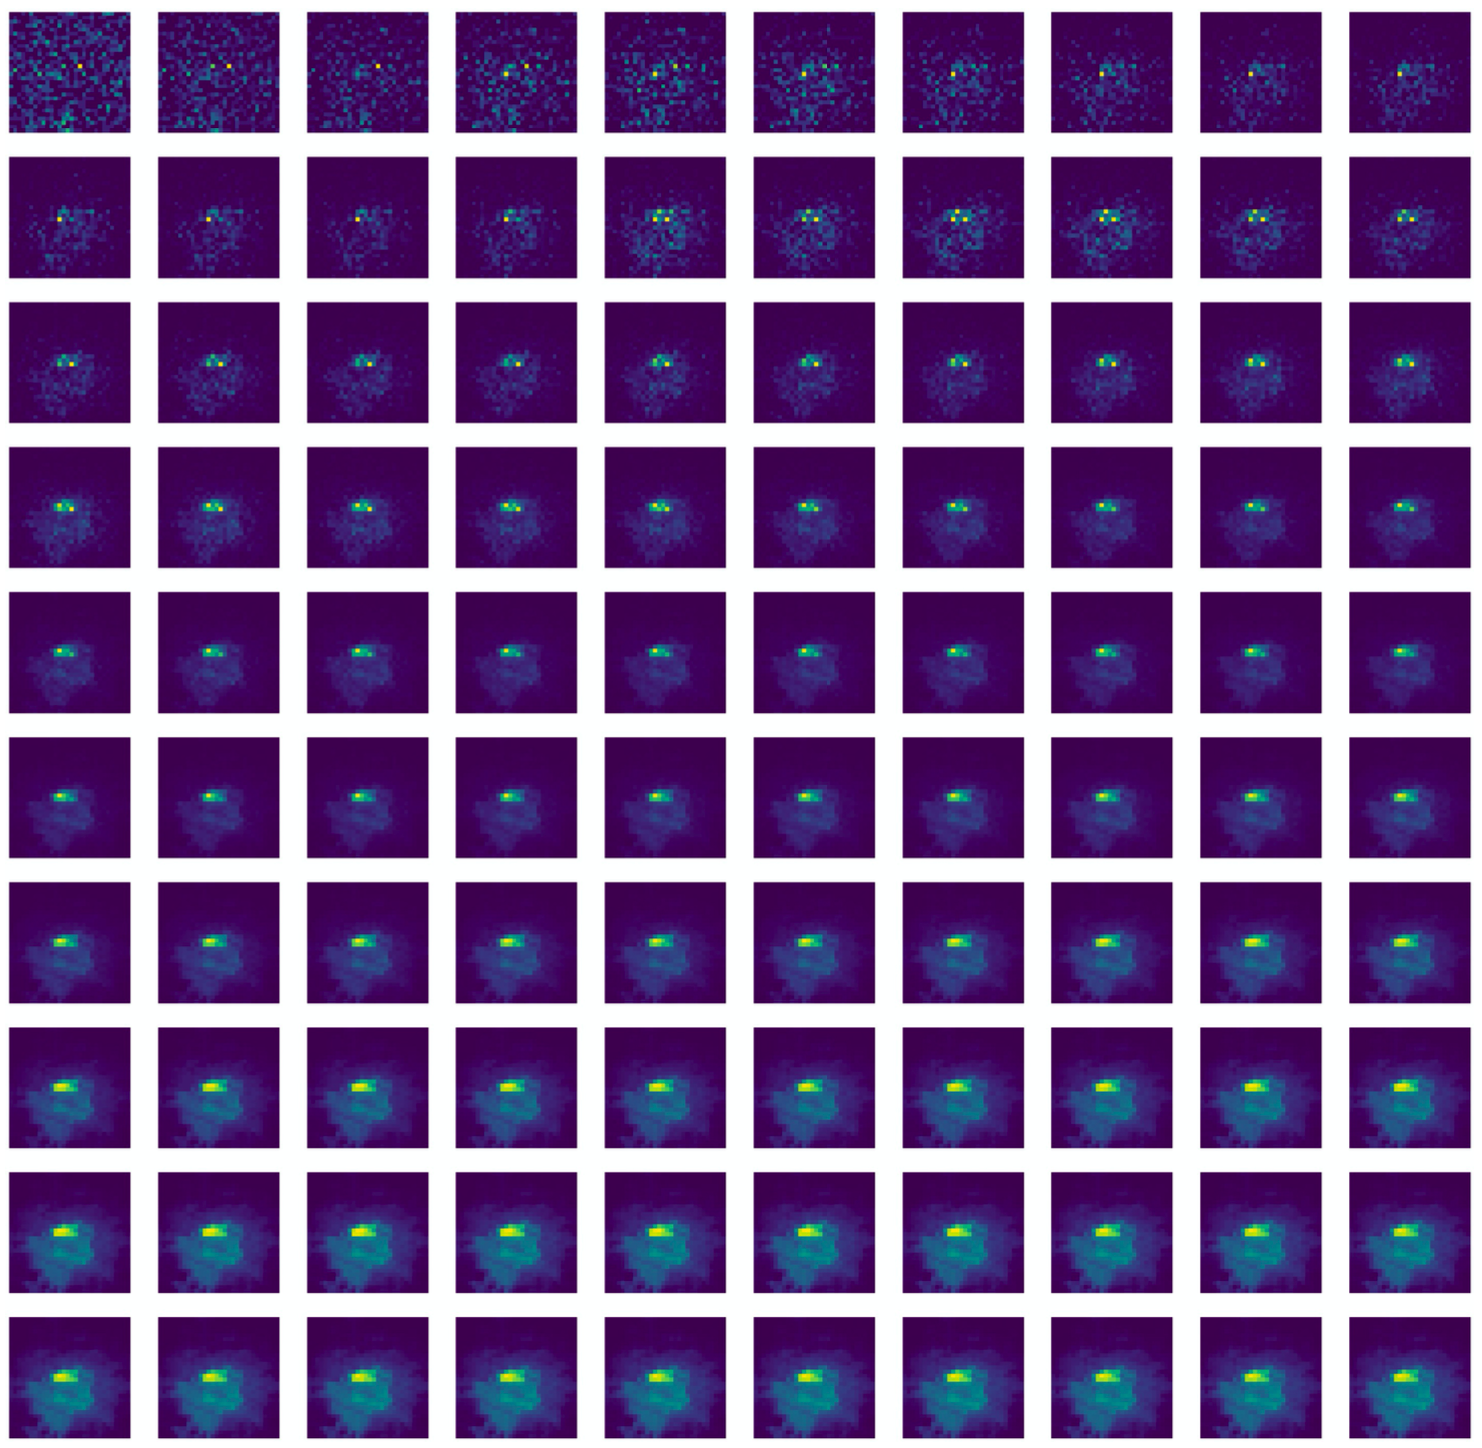
\includegraphics[width = 0.8\linewidth]{pics/simu.png}
        \caption{A simulation}
    \end{figure}
\end{frame}